% res_timing.tex  -- written by Saumya
\subsection{Effect of Overlapping}
Fig.~\ref{fig:wave} shows three consecutive products in overlapped mode.
While the controller is in \textsc{Clear}/\textsc{Feed}/\textsc{Drain}, the
host writes the next $A$ and $B$ (\texttt{wr\_en}) into the inactive bank and
reads the previous result (\texttt{rd\_row} 0--3). A \texttt{done} pulse
occurs every 12 cycles, and the bank pointer alternates.

\begin{figure*}[t]
\centering
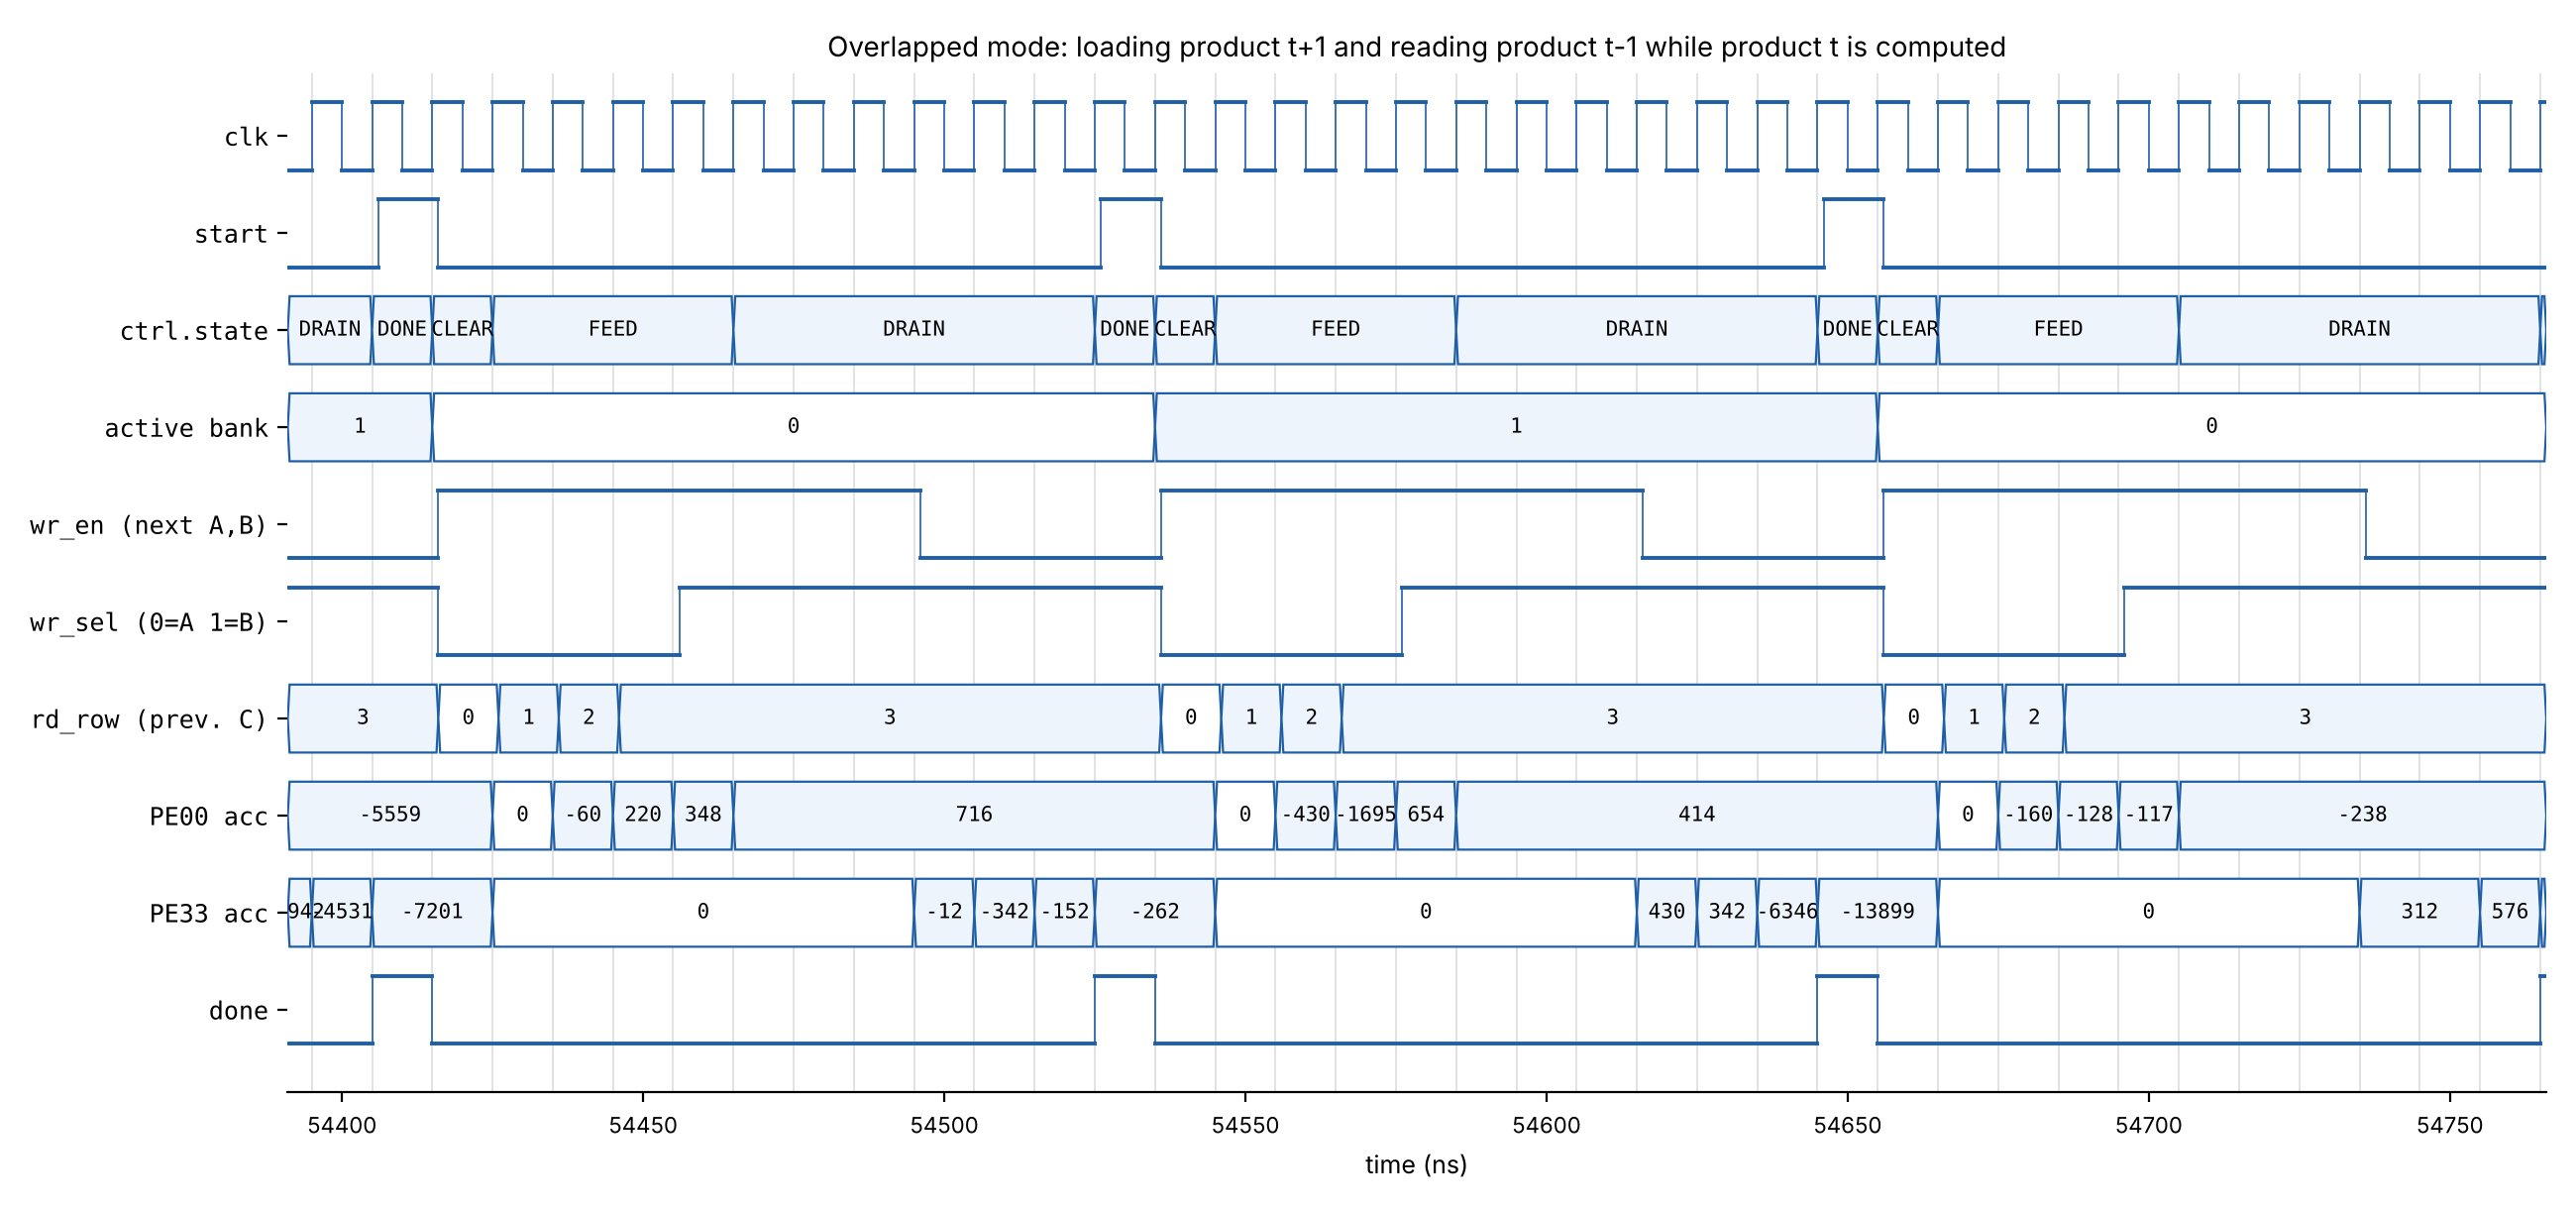
\includegraphics[width=0.95\textwidth]{fig_wave_v2.png}
\caption{Overlapped (streaming) operation of \texttt{systolic\_top\_v2}: host transfers for products $t\pm1$ happen while product $t$ is computed.}
\label{fig:wave}
\end{figure*}

\subsection{Timing Closure and Pipelining}
Without extra registers the design reaches only 51.3~MHz, although an
isolated MAC closes at 193~MHz. The nextpnr critical path runs from the
controller state register, through the feed decode and the buffer read
multiplexer, into the PE$(0,0)$ multiplier and its 32-bit adder. Lane~0 of
the skew logic has no register, so all of these are in series.
Table~\ref{tab:pipe} and Fig.~\ref{fig:pipe} show the effect of the two
optional registers. Each adds one cycle of latency (12$\to$14 cycles per
product) but shortens the critical path. Together they raise $f_{\max}$ by
2.27$\times$ and cut the time per product from 235 to 121~ns. After both
registers, the remaining critical path is one PE forwarding register
feeding the neighbouring DSP multiplier, which is the natural limit of
this structure.

\begin{table}[t]
\centering
\caption{Pipelining study ($N=4$, overlapped, ECP5 post-route)}
\label{tab:pipe}
\setlength{\tabcolsep}{3pt}
\begin{tabular}{@{}lrrrrr@{}}
\toprule
\textbf{registers} & \textbf{latency} & \textbf{cyc/prod} & \textbf{$f_{\max}$} & \textbf{ns/prod} & \textbf{LUT}\\
\midrule
none        & 12 & 12.06 & 51.3  & 235 & 2534 \\
MAC pipe    & 13 & 13.06 & 76.2  & 171 & 3424 \\
buffer reg  & 13 & 13.06 & 70.6  & 185 & 3000 \\
both        & 14 & 14.06 & 116.4 & 121 & 3522 \\
\bottomrule
\end{tabular}
\end{table}

\begin{figure}[t]
\centering
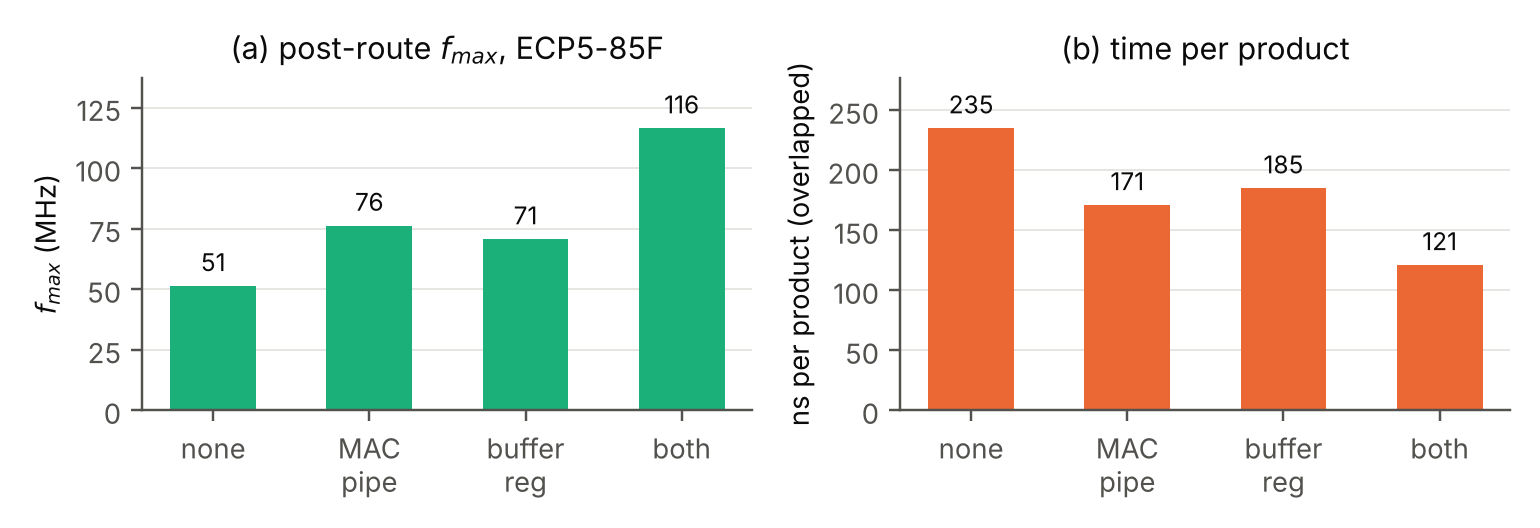
\includegraphics[width=\columnwidth]{fig_pipeline.png}
\caption{(a) Post-route $f_{\max}$ and (b) time per product for each pipeline option.}
\label{fig:pipe}
\end{figure}

\subsection{FPGA Resource Utilisation}
Table~\ref{tab:synth} lists synthesis results. On Xilinx 7-series, Yosys
maps each MAC into one DSP48E1 slice, using the slice's own post-adder as
the accumulator. Without DSPs (\texttt{-nodsp}) a single MAC costs 339
LUTs instead of 32. Phase~II roughly doubles the flip-flops of Phase~I: the
two operand banks add 512~FFs and the result buffer another 512. This is
the price of overlapping. At $N=8$ the design needs 64 DSPs and
10.8\,k LUTs, which still fits a mid-range Artix-7 (e.g.\ XC7A100T with 240
DSPs). The 90 DSPs of an XC7A35T limit that device to $N\le 9$.

\begin{table}[t]
\centering
\caption{Synthesis results (Xilinx 7-series via Yosys; ECP5 post-route via nextpnr)}
\label{tab:synth}
\setlength{\tabcolsep}{2.2pt}
\begin{tabular}{@{}lrrrrr@{}}
\toprule
\textbf{Design} & \textbf{LUT} & \textbf{FF} & \textbf{DSP} & \textbf{ECP5 LUT4} & \textbf{$f_{\max}$}\\
\midrule
MAC (comb.)        & 32    & 32   & 1  & 103   & 193.1 \\
MAC (pipelined)    & 64    & 50   & 1  & 121   & 208.7 \\
MAC, no DSP        & 339   & 32   & 0  & --    & -- \\
Sequential base.   & 82    & 40   & 1  & 203   & 75.7 \\
Phase~I top        & 1535  & 1064 & 16 & 4894  & 55.5 \\
v2, $N=2$          & 842   & 567  & 4  & 2714  & 66.7 \\
v2, $N=4$          & 2534  & 1961 & 16 & 7740  & 51.3 \\
v2, $N=4$, fast    & 3522  & 2284 & 16 & 8034  & 116.4 \\
v2, $N=8$          & 10835 & 7627 & 64 & 29396 & -- \\
WS, $N=4$          & 32    & 859  & 16 & 1269  & 82.9 \\
\bottomrule
\end{tabular}
\end{table}
